\documentclass[convert={density=150x150},border={10pt 10pt 10pt 10pt}]{standalone}
\usepackage{amsmath, amssymb, amsthm}
\usepackage{tikz}
\usetikzlibrary{arrows,shapes,snakes,automata,backgrounds,petri}
\usetikzlibrary{positioning,decorations.text}
\tikzset{n/.style={inner sep=0, minimum size=6pt, fill=black, circle}}
\begin{document}
\pagecolor{white}
  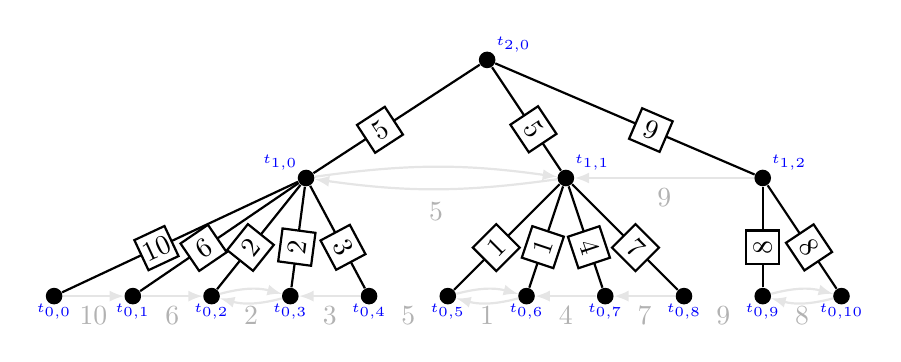
\begin{tikzpicture}
    \foreach \x in {0,1,...,10}
    {
      \node[n,label={[label distance=-4pt]270:{\color{blue}{\tiny$t_{0,\x}$}}}](A\x) at (\x, 0) {};
    }
    \node[n,label={[label distance=-4pt]120:{\color{blue}{\tiny$t_{1,0}$}}}](B1) at (3.2, 1.5) {};
    \node[n,label={[label distance=-4pt]75:{\color{blue}{\tiny$t_{1,1}$}}}](B2) at (6.5, 1.5) {};
    \node[n,label={[label distance=-4pt]75:{\color{blue}{\tiny$t_{1,2}$}}}](B3) at (9, 1.5) {};

    \def\testarray{{10,6,2,2,3,1,1,4,7,8,8}}
    \foreach \x in {0,1,2,3,4}{
      \pgfmathparse{\testarray[\x]}
      \edef\v{\pgfmathresult}
      \draw[black,thick,sloped] (A\x) -- (B1) node [fill=white,draw=black,inner sep=0,minimum size=12pt, pos=0.4] {$\v$};
      %\draw[black!50,thick,postaction={decorate,decoration={text along path, text={$\v$}, text align={center}}}] (A\x) -- (B1);
    }
    \foreach \x in {5,6,7,8}{
      \pgfmathparse{\testarray[\x]}
      \edef\v{\pgfmathresult}
      \draw[black,thick,sloped] (A\x) -- (B2) node [fill=white,draw=black,inner sep=0,minimum size=12pt, pos=0.4] {$\v$};
    }

    \foreach \x in {9,10}{
      \pgfmathparse{\testarray[\x]}
      \edef\v{\pgfmathresult}
      \draw[black,thick,sloped] (A\x) -- (B3) node [fill=white,draw=black,inner sep=0,minimum size=12pt, pos=0.4] {$\v$};
    }

    \node[n,label={[label distance=-4pt]75:{\color{blue}{\tiny$t_{2,0}$}}}](C1) at (5.5, 3) {};
    \def\higherarray{{0,5,5,9}}
    \foreach \x in {1,2,3}{
      \pgfmathparse{\higherarray[\x]}
      \edef\v{\pgfmathresult}
      \draw[black,thick,sloped] (B\x) -- (C1) node [fill=white,draw=black,inner sep=0,minimum size=12pt, pos=0.4] {$\v$};
    }

     
    \def\origarray{{10,6,2,3,5,1,4,7,9,8}}
    \foreach \x in {0,1,...,9}
    {
      \pgfmathparse{int(\x+1)}
      \edef\y{\pgfmathresult}%
      \pgfmathparse{\origarray[\x]}
      \edef\v{\pgfmathresult}
      \draw[opacity=0,thick,text opacity=1] (A\x) -- (A\y) node [black!30, midway, below] {$\v$};
    }
    \foreach \x in {0,1} {
      \pgfmathparse{int(\x+1)}
      \edef\y{\pgfmathresult}%
      \draw[black!10, -latex,thick] (A\x) edge (A\y);
    }
    \foreach \x in {2,5,9} {
      \pgfmathparse{int(\x+1)}
      \edef\y{\pgfmathresult}%
      \draw[black!10, -latex,thick] (A\x) edge [bend left=15] (A\y);
      \draw[black!10, -latex,thick] (A\y) edge [bend left=15] (A\x);
    }
    \foreach \x in {3,6,7} {
      \pgfmathparse{int(\x+1)}
      \edef\y{\pgfmathresult}%
      \draw[black!10, -latex,thick] (A\y) edge (A\x);
    }
    %\draw[rounded corners,draw=red,thick] (-0.2, -0.2) rectangle (4.2, 0.2);
    %\draw[rounded corners,draw=red,thick] (4.8, -0.2) rectangle (8.2, 0.2);
    %\draw[rounded corners,draw=red,thick] (8.8, -0.2) rectangle (10.2, 0.2);


    %\draw[thick, dashed, draw=red, -latex](B1) edge [red, bend right] (4, 0.3);
    %\draw[thick, dashed, draw=red, -latex](B2)-- (6, 0.3);
    %\draw[thick, dashed, draw=red, -latex](B3) edge [red, bend left] (9, 0.3);
    \draw[opacity=0,text opacity=1,black!10,thick] (B1)--(B2) node[black!30, midway, below, yshift=-5pt] {$5$};
    \draw[black!10,thick, -latex] (B3) -- (B2) node[black!30, midway, below] {$9$};
    \draw[thick] (B1) edge[black!10,bend left=8, -latex] (B2);
    \draw[thick] (B2) edge[black!10,bend left=8, -latex] (B1);
    %\draw[rounded corners,draw=red,thick] (4.8, 1.3) rectangle (7.2, 1.7);
  \end{tikzpicture}
\end{document}